\chapter{Background}
\label{chap:background}

Questo capitolo introduce le tecnologie, i paradigmi ed i concetti fondamentali
necessari per la compensione del contributo della tesi.
In apertura si delineano i principi dell'Aggregate Computing, con particolare
attenzione all'implementazione nel contesto dei dispositivi con risorse limitate.
Successivamente, si presentano il framework \ac{YAAIR}, il protocollo di rete
Zenoh \footnote{\url{https://zenoh.io/}} ed il relativo ecosistema per sistemi embedded.
In conclusione, viene fatta un'analisi delle tecnologie Rust necessarie per la
programmazione e compilazione \emph{cross-platform} su architetture hardware
eterogenee.

\section{Aggregate computing}
\label{sec:aggregate-computing}
Il rapido proliferare di dispositivi per lo \ac{IoT} e di sistemi di
calcolo pervasivo ha generato sfide senza precedenti nella programmazione e nel
coordinamento di sistemi altamente distribuiti.
Gli approcci di programmazione tradizionali faticano a gestire la complessità
derivante dalla necessità di far cooperare centinaia o migliaia di dispositivi
in modo trasparente e resiliente~\cite[12.1]{10.1007/978-3-031-95589-1_12}.
\note{Questo primo paragrafo è praticamente la traduzione parola per parola della
sezione citata del vostro paper: devo mettere la citazione in qualche modo per far
capire che è esattamente lo stesso testo?}

\subsection{Modello computazionale}
\label{ssec:ac-computational-model}

Lo \ac{AC} si impone come un paradigma di \emph{macroprogrammazione}~\cite{enwiki:1313791910}
che astrae l'esecuzione di un singolo programma su una rete di dispositivi
considerandola come un'unica entità collettiva.
Al centro di questo modello vi sono il \emph{field calculus} ed i \emph{campi computazionali}, astrazioni che mappano punti nello spazio e nel tempo a valori
che possono essere combinati funzionalmente~\cite[12.2.1]{10.1007/978-3-031-95589-1_12}.
Ad esempio, in uno sciame robotico, si possono definire diversi campi computazionali
che associano ad ogni robot un valore come la distanza minima da una sorgente o
un vettore rappresentante il movimento desiderato~\cite[2.1.2, ACV25]{amslaurea37138}.

Ogni dispositivo nel sistema raccoglie dati dal proprio stato locale e dai vicini,
calcola il programma aggregato costruendo un risultato da esportare, ed infine
attua il risultato del calcolo ed invia il proprio risultato ai dispositivi con
cui è in relazione~\cite[2.1.1]{amslaurea37138}.

Un esempio classico di questa computazione è la costruzione di un gradiente spaziale,
utilizzato per misurare la distanza di ogni nodo da una sorgente, dove le relazioni
tra i nodi sono basate sul concetto di vicinato definito distanza cartesiana tra
loro~\cite[12.2.2]{10.1007/978-3-031-95589-1_12}~(\Cref{fig:gradient_ac}).

\begin{figure}[htpb]
    \centering
    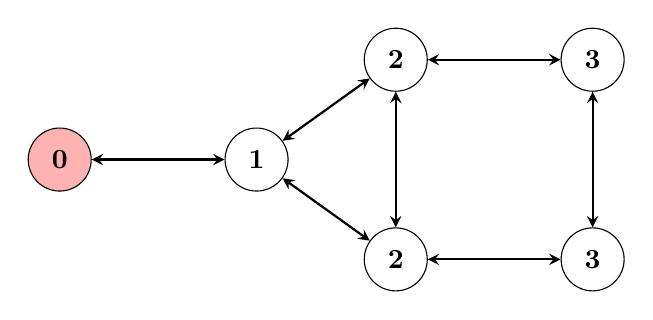
\begin{tikzpicture}[
        >=stealth,
        node distance=2.5cm,
        every node/.style={circle, draw, minimum size=8mm, font=\bfseries},
        edge/.style={draw, thick, <->}
    ]
        \node[fill=red!30] (S) {0};
        \node (A) [right of=S] {1};
        \node (B) [above right of=A, yshift=-0.5cm] {2};
        \node (C) [below right of=A, yshift=0.5cm] {2};
        \node (D) [right of=B] {3};
        \node (E) [right of=C] {3};

        \path[edge] (S) -- (A);
        \path[edge] (A) -- (B);
        \path[edge] (A) -- (C);
        \path[edge] (B) -- (C);
        \path[edge] (B) -- (D);
        \path[edge] (C) -- (E);
        \path[edge] (D) -- (E);
    \end{tikzpicture}
    \caption{Rappresentazione di un gradiente spaziale in un sistema distribuito.
    Il nodo sorgente (in rosso) ha distanza 0, mentre i nodi adiacenti calcolano
    la propria distanza propagando il valore attraverso il vicinato.}
    \label{fig:gradient_ac}
\end{figure}

\subsection{Aggregate computing su sistemi embedded}
\label{ssec:ac-on-embedded-devices}

Il modello di computazione distribuita che offre il paradigma dello \ac{AC} si
pone come soluzione naturale per reti di dispositivi \ac{IoT} e sciami robotici.
Framework preesistenti, come ScaFi (basato su Scala~\cite{itwiki:144756110})~\cite[2.3]{amslaurea37138},
sono stati concepiti per simulazioni o esecuzioni su dispositivi general-purpose,
il che li rende incompatibili con i microcontrollori a basso costo per l'assenza
di memoria sufficiente e garanzie real-time.
Un programma aggregato deve operare in esecuzione asincrona e continua,
richiedendo una gestione deterministica della memoria e un accesso efficiente ai
protocolli di rete.

In questo scenario, il linguaggio Rust~\cite{itwiki:149175104} rappresenta una soluzione
architetturale ideale: grazie al suo modello di \emph{ownership} e all'assenza di
\ac{GC}, Rust fornisce astrazioni a costo zero garantendo prestazioni predicibili,
latenze minime e una sicurezza della memoria fondamentale per la programmazione
embedded.

\section{YAAIR}
\label{sec:yaair}

\ac{YAAIR} \footnote{\url{https://github.com/nicolasfara/yaair}} è un framework
Rust open-source per lo \ac{AC}, ideato per risolvere le limitazioni prestazionali
dei framework basati su linguaggi ad alto livello che non permettono l'esecuzione
su sistemi embedded.
Sfruttando la natura flessibile di Rust data dal concetto di \emph{trait},
\ac{YAAIR} propone un modello architetturale a strati che disaccoppia la logica
di calcolo del programma aggregato dalla serializzazione e dai protocolli di rete
sottostanti. Questo livello di isolamento consente al sistema di operare indipendentemente
dall'hardware, eseguendo cicli di valutazione in modo totalmente agnostico rispetto
al trasporto fisico dei dati.

Il contributo di questa tesi si concentra sull'implementazione di una alternativa
decentralizzata per lo strato di rete basata sul protocollo Zenoh.

\section{Zenoh}
\label{sec:zenoh}

Zenoh è un protocollo emergente e un'infrastruttura di rete decentralizzata per
la comunicazione \emph{pub/sub/query}, orientato a latenze minime e scalabilità
su dispositivi eterogenei.
A differenza di protocolli tradizionali dell'ecosistema \ac{IoT} come \ac{MQTT}
\footnote{\url{https://mqtt.org/}}, che si appoggiano obbligatoriamente ad un
broker centrale (creando colli di bottiglia e un singolo punto di fallimento),
Zenoh è progettato per unificazioni \emph{edge-to-cloud} senza vincoli topologici
stretti~\cite{zenoh:what-is-zenoh}.

\subsection{Modello di comunicazione}
\label{ssec:zenoh-communication-model}

Il modello di Zenoh adotta un approccio ibrido altamente flessibile, basato
essenzialmente su architetture \ac{P2P}. I nodi sulla rete possono
assumere ruoli differenziati:

\begin{itemize}
    \item \textbf{Client}: Dispositivi con risorse minime, che si connettono ai
    router o ad altri peer per l'inoltro dei pacchetti senza occuparsi della
    topologia di routing globale.
    \item \textbf{Peer}: Nodi in grado di comunicare in maniera diretta fra loro
    e di gestire topologie P2P auto-organizzanti grazie a meccanismi integrati
    di scoperta automatica dei nodi nella rete (\emph{scouting}).
    \item \textbf{Router}: Elementi strutturali utilizzati per unire reti isolate
    o scalare la topologia su geografie estese.
\end{itemize}

Tale flessibilità sposa perfettamente i requisiti dei sistemi aggregati in cui
il fallimento di un nodo non deve compromettere l'intera struttura di comunicazione
del vicinato.

\subsection{Attori e concetti fondamentali}
\label{ssec:zenoh-actors-and-fundamental-concepts}

A livello applicativo, la comunicazione in Zenoh avviene all'interno di una
\emph{Sessione}, la quale incapsula la connettività del nodo. Sfruttando un
approccio incentrato sui dati, l'indirizzamento è dettato tramite \emph{Key
Expressions}, permettendo a molteplici entità di registrarsi sugli stessi topic.

Zenoh permette di utilizzare modelli di comunicazione \emph{pub/sub} e \emph{query/reply}
in maniera ibrida all'interno della stessa sessione, definendo rispettivamente
\emph{Publishers} che pubblicano dati su topic specifici a cui i \emph{Subscribers}
possono iscriversi o \emph{Queryables} che rispondono a richieste effettuate attivamente
da \emph{Queriers} in una comunicazione più simile al modello \ac{RPC}.

\section{Zenoh per sistemi embedded}
\label{ssec:zenoh-for-embdedded-systems}

Nonostante la flessibilità di Rust come linguaggio che ne permette l'utilizzo
anche per la programmazione di dispositivi \emph{bare-metal}, come diversi dispositivi
utilizzati per la programmazione \ac{IoT}, Zenoh come libreria dipende da alcune
funzionalità specifiche che richiedono la presenza di un sistema operativo completo
sul dispositivo.

Per colmare questa lacuna è stato introdotto Zenoh pico \footnote{\url{https://github.com/eclipse-zenoh/zenoh-pico}},
un porting leggero della libreria in C appositamente concepito per sistemi embedded
dotati di vincoli severi.
Questa versione copre quasi completamente le funzionalità della libreria originale,
omettendo la possibilità di utilizzare un nodo come \emph{router}
(\cref{ssec:zenoh-communication-model}).

Si menziona, a corredo dell'ecosistema, il nascente progetto \texttt{zenoh-nostd}
\footnote{\url{https://github.com/ZettaScaleLabs/zenoh-nostd}}, un'iniziativa
volta a fornire un porting interamente in Rust senza dipendenze dalla libreria standard.
Tuttavia, trovandosi ancora in una fase sperimentale, per la creazione del contributo
di questa tesi è stato utilizzato Zenoh pico creando un wrapper Rust per la libreria.

\section{Embedded Rust}
\label{ssec:embedded-rust}

Per mitigare le discrepanze tra le piattaforme di testing (computer x86/ARM completi)
e il dominio di attuazione robotico, Rust si presenta come ecosistema duale.
Questo bivalente modello si adatta particolarmente all'astrazione hardware, requisito
centrale nell'orchestrazione aggregata che postula l'agnosticismo della piattaforma,
dove robot con piattaforme differenti dovrebbero poter unirsi al team in modo flessibile
\cite{10.1007/978-3-031-95589-1_12}[cite: 154].

\subsection{Cross-compilation}
\label{ssec:cross-compilation}

L'infrastruttura di Cargo e \texttt{rustc} abilita la compilazione multipiattaforma
mediante pattern di \emph{conditional compilation}. L'aggiunta di \emph{toolchain}
specifiche (es. \texttt{nightly}) accoppiate alla feature \texttt{build-std}
permette di generare binari compilati dal sorgente base per target come architetture
RISC-V o Xtensa. Questo approccio è esplicitato attraverso direttive condizionali
in Rust, che attivano moduli diversi in fase di build dipendentemente dall'OS
target (e.g., \texttt{\#[cfg(target\_os = "espidf")]}), permettendo una vera e
propria architettura a doppia implementazione.

% \begin{lstlisting}[language=Rust, caption={Esempio di compilazione condizionale per l'architettura di rete YAAIR}, label={lst:cfg_zenoh}]
% #[cfg(zenoh_impl = "zenoh_full")]
% #[path = "zenoh_full/mod.rs"]
% mod zenoh_impl;

% #[cfg(zenoh_impl = "zenoh_pico")]
% #[path = "zenoh_pico/mod.rs"]
% mod zenoh_impl;
% \end{lstlisting}

\subsection{ESP-IDF}
\label{ssec:esp-idf}

Per i dispositivi basati sui chip Espressif (come ESP32), l'ambiente Embedded
Rust sfrutta comunemente un bridge diretto con l'Espressif IoT Development Framework
(ESP-IDF). Invece di adottare un approccio puramente \emph{bare-metal}
(\texttt{no\_std}), la compilazione tramite l'ecosistema \texttt{esp-idf-sys}
permette di dotare la CPU di una sottile implementazione della libreria standard
di Rust, garantendo l'accesso ad allocatori heap globali e threading gestito
dall'RTOS (FreeRTOS) fornito da Espressif.

\subsubsection{Interazione con l'hardware}
\label{sssec:hardware-interaction}

L'astrazione fornita dai crate legati a ESP-IDF permette l'interazione type-safe
con le periferiche hardware del microcontrollore. Il Wi-Fi, critico per la
costituzione della rete di Zenoh, i pin GPIO, i timer e i canali I2C/SPI per
l'attuazione cinetica, vengono mappati su struct Rust. Qualora la sicurezza non
possa essere garantita a livello di compilatore (come nelle modifiche hardware
concorrenti), la responsabilità è mediata da primitivi di sincronizzazione o
passaggi di possesso espliciti.

\subsubsection{Componenti e librerie esterne}
\label{sssec:components-and-external-libraries}

Un vantaggio sostanziale dell'architettura ESP-IDF in Rust risiede nella capacità
di registrare librerie C come \emph{extra components} durante il processo di build
basato su CMake. Nel contesto della tesi, questo paradigma ingegneristico è vitale:
la libreria C \texttt{zenoh-pico} viene configurata come modulo esterno, in modo
che l'infrastruttura di build di ESP-IDF la compili nativamente per l'architettura
target, estraendo contestualmente i binding sicuri per Rust tramite utilità come
\texttt{bindgen}.

\subsection{Embassy}
\label{sec:embassy}

Infine, l'esecuzione in background di task legati allo scouting di rete, alla
ricezione costante di messaggi tramite callback di Zenoh e ai cicli computazionali
di YAAIR necessita di un approccio concorrente efficiente. Al fine di evitare i
costi dei thread di sistema tradizionali, la libreria \textbf{Embassy} ricopre
il ruolo di runtime asincrono moderno progettato esclusivamente per sistemi embedded.
Sfruttando la generazione di macchine a stati finiti in fase di compilazione fornita
da Rust Asincrono, Embassy assicura un'esecuzione efficiente del codice logico
senza bloccaggi dell'OS sottostante, minimizzando il consumo energetico e
abilitando, ad esempio, l'invio reattivo di pacchetti \emph{heartbeat} per
notificare la presenza dinamica dei nodi all'interno dello sciame \ac{P2P}.
